\documentclass[11pt,letterpaper,twocolumn]{fenbil}

\begin{document}
\twocolumn[\begin{@twocolumnfalse}

\begin{minipage}{0.15\textwidth}{
    
\includegraphics[width=4cm]{logo/iufizik.png}}
\end{minipage}
\hspace{25pt}
\begin{minipage}{0.75\textwidth}
\vspace{5mm}
    \Large{\textbf{Fresnel Eşitlikleri ve Yansıma Teorisi Deney Raporu
     }}
    \vspace{3mm}
    
    \large{\textbf{Ad Soyad}; Celal Ekrem Torun - 0411230037} 
    \vspace{2mm}
    
    \large{\textbf{Danışman: }Arş. Gör. Ömer Göksel ERBAŞ}\newline
    \fontsize{0.35cm}{0.5cm}\selectfont \textit{Fizik Bölümü, İstanbul Üniversitesi\newline 
    Beyazıt, Fatih, İstanbul, Türkiye\newline
    5 Mart, 2025}
    
\end{minipage}

\small

\end{@twocolumnfalse}]

\section*{1. Amaç}
Bu deneyin amacı, düzlem polarize ışığın bir yüzeye farklı açılarda yansıtılmasıyla meydana gelen polarizasyon dönüşümünü incelemek ve yansıyan ışık şiddetini ölçmektir. Ayrıca, elde edilen deneysel sonuçları Fresnel formülleriyle karşılaştırarak teorinin geçerliliğini test etmek ve yüzeyin kırılma indisini belirlemektir. Bu doğrultuda, dikey ve yatay polarize ışığın farklı geliş açılarında yansıma davranışlarını gözlemleyip, Brewster açısını deneysel olarak tespit etmek de deneyin amaçları arasındadır.

\section*{2. Teorik Bilgi}
Işık, elektromanyetik dalgalar olarak modellenebilir ve bu dalgaların polarizasyonu, elektrik alan vektörünün yönü ile tanımlanır. Bir ortamdan diğerine geçişte, ışık hem yansıma hem de kırılma davranışı sergiler. Bu davranışlar, Fresnel eşitlikleri tarafından matematiksel olarak ifade edilir.

\subsection*{2.1. Fresnel Eşitlikleri}
Fresnel eşitlikleri, polarize ışığın bir yüzeyden yansıması ve kırılması sırasında meydana gelen şiddet değişimlerini açıklar. Bu eşitlikler, gelen ışığın polarizasyonuna bağlı olarak iki farklı formda ifade edilir:

\subsubsection*{2.1.1. Dikey (s-polarize) Işık İçin}
Gelen ışığın elektrik alan vektörü, geliş düzlemine dik olduğunda, yansıma katsayısı aşağıdaki formülle hesaplanır:
\[
r_s = \frac{n_1 \cos{\theta_i} - n_2 \cos{\theta_t}}{n_1 \cos{\theta_i} + n_2 \cos{\theta_t}}
\]

Buna bağlı olarak, yansıma şiddeti:
\[
R_s = |r_s|^2 = \left(\frac{n_1 \cos{\theta_i} - n_2 \cos{\theta_t}}{n_1 \cos{\theta_i} + n_2 \cos{\theta_t}}\right)^2
\]

\subsubsection*{2.1.2. Yatay (p-polarize) Işık İçin}
Gelen ışığın elektrik alan vektörü, geliş düzlemine paralel olduğunda, yansıma katsayısı:
\[
r_p = \frac{n_2 \cos{\theta_i} - n_1 \cos{\theta_t}}{n_2 \cos{\theta_i} + n_1 \cos{\theta_t}}
\]

Yansıma şiddeti:
\[
R_p = |r_p|^2 = \left(\frac{n_2 \cos{\theta_i} - n_1 \cos{\theta_t}}{n_2 \cos{\theta_i} + n_1 \cos{\theta_t}}\right)^2
\]

Burada:
\begin{itemize}
    \item \( n_1 \): İlk ortamın kırılma indisi (genellikle hava için \( n_1 \approx 1 \))
    \item \( n_2 \): İkinci ortamın kırılma indisi
    \item \( \theta_i \): Geliş açısı
    \item \( \theta_t \): Kırılma açısı (Snell Yasası ile \( n_1 \sin{\theta_i} = n_2 \sin{\theta_t} \) olarak hesaplanır)
\end{itemize}

\subsection*{2.2. Brewster Açısı}
Brewster açısı, yatay polarize ışığın (p-polarize) yansıma katsayısının sıfır olduğu açıdır. Bu durumda, yansıyan ışık tamamen dikey polarize olur. Brewster açısı şu şekilde hesaplanır:
\[
\theta_B = \arctan{\left(\frac{n_2}{n_1}\right)}
\]

\subsection*{2.3. Snell Yasası}
Işığın bir ortamdan diğerine geçişinde kırılma açısını veren Snell Yasası:
\[
n_1 \sin{\theta_i} = n_2 \sin{\theta_t}
\]

\subsection*{2.4. Optik Yoğunluk ve Kırılma İndisi}
Bir malzemenin optik yoğunluğu, ışığın o malzeme içindeki hızını belirler. Kırılma indisi, ışığın boşluktaki hızının malzeme içindeki hızına oranıdır:
\[
n = \frac{c}{v}
\]

Burada:
\begin{itemize}
    \item \( n \): Kırılma indisi
    \item \( c \): Işığın boşluktaki hızı (\( 3 \times 10^8 \) m/s)
    \item \( v \): Işığın malzeme içindeki hızı
\end{itemize}

\section*{3. Deneyin Yapılışı}
\begin{enumerate}
    \item Deney düzeneği kuruldu: ışık kaynağı, polarizör, cam yüzey ve fotodetektör yerleştirildi.
    \item Işık kaynağından çıkan ışın bir polarizör yardımıyla önce dikey (s-polarize) sonra yatay (p-polarize) olarak polarize edildi.
    \item Cam yüzey, ışık kaynağına göre 0° ile 80° arasında değişen açılarda konumlandırıldı.
    \item Her bir açıda ve polarizasyon durumunda, yansıyan ışığın şiddeti fotodetektör yardımıyla ölçüldü.
    \item Elde edilen şiddet değerleri kaydedildi ve bu değerler kullanılarak grafikler oluşturuldu.
    \item Brewster açısını belirlemek için, p-polarize ışığın yansıma şiddetinin minimum olduğu açı tespit edildi.
    \item Deneysel sonuçlar, Fresnel eşitlikleri kullanılarak hesaplanan teorik değerlerle karşılaştırıldı.
\end{enumerate}

\section*{4. Ölçüm Sonuçları}
\begin{table}[H]
    \begin{center}
        \resizebox{8.25cm}{!}{
            \begin{tabular}{|c|c|c|}
            \hline
            \textbf{Açı (°)} & \textbf{Dikey Polarizasyon (I)} & \textbf{Yatay Polarizasyon (I)} \\ \hline
            0 & 37 & 124.3 \\ \hline
            10 & 3.3 & 120 \\ \hline
            15 & 2.5 & 120 \\ \hline
            20 & 2 & 110 \\ \hline
            25 & 2.3 & 96 \\ \hline
            30 & 2.5 & 120 \\ \hline
            40 & 2.3 & 80 \\ \hline
            45 & 2.6 & 43 \\ \hline
            50 & 2.5 & 5 \\ \hline
            52.5 & 2.3 & 4 \\ \hline
            55 & 2 & 1.1 \\ \hline
            57 & 2.4 & 2.3 \\ \hline
            58 & 4.3 & 1.4 \\ \hline
            60 & 2.2 & 2.6 \\ \hline
            65 & 6.6 & 28 \\ \hline
            70 & 9.7 & 105 \\ \hline
            75 & 15.2 & 126 \\ \hline
            80 & 19.7 & 125 \\ \hline
            \end{tabular}
        }
    \end{center}
    \caption{Farklı geliş açıları için dikey ve yatay polarize ışık şiddetleri.}
\end{table}

\begin{figure}[H]
    \begin{center}
        \resizebox{8.25cm}{!}{
            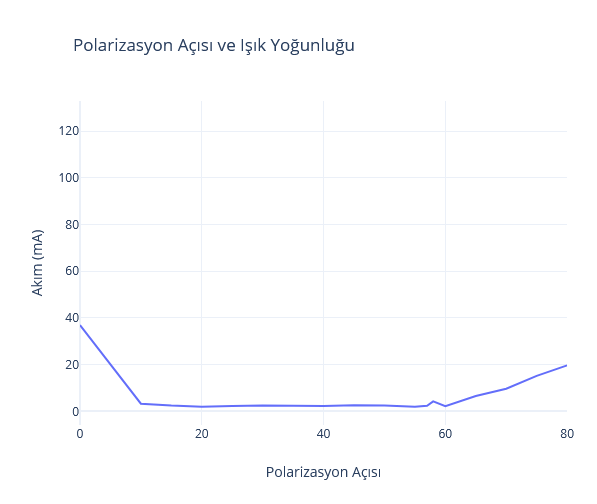
\includegraphics{graph/dikey_polarizasyon.png}
        }
    \end{center}
    \caption{Dikey Polarizasyon için Yansıma Şiddeti - Açı Grafiği} 
    \label{fig:dikey}
\end{figure}

\begin{figure}[H]
    \begin{center}
        \resizebox{8.25cm}{!}{
            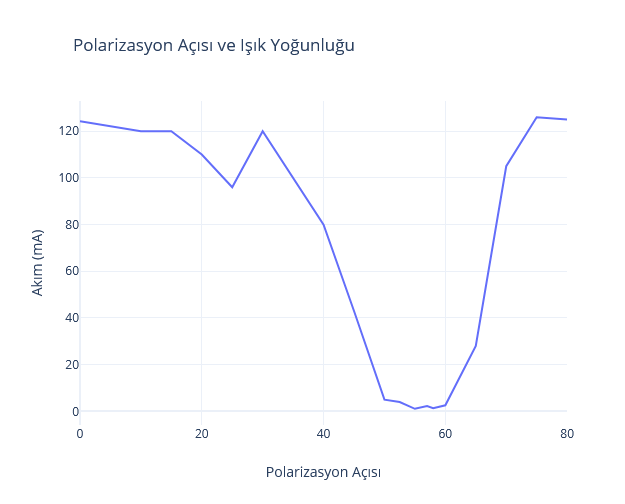
\includegraphics{graph/yatay_polarizasyon.png}
        }
    \end{center}
    \caption{Yatay Polarizasyon için Yansıma Şiddeti - Açı Grafiği} 
    \label{fig:yatay}
\end{figure}

\begin{figure}[H]
    \begin{center}
        \resizebox{8.25cm}{!}{
            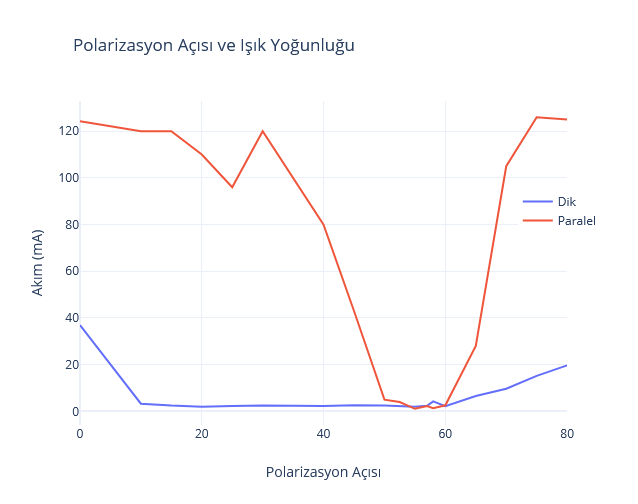
\includegraphics{graph/karsilastirma.png}
        }
    \end{center}
    \caption{Dikey ve Yatay Polarizasyon için Yansıma Şiddetlerinin Karşılaştırma Grafiği} 
    \label{fig:karsilastirma}
\end{figure}

\section*{5. Hesaplamalar}
Aşağıda, elde edilen veriler üzerinde yapılan hesaplamalar ve analizler sunulmuştur.

\subsection*{5.1. Brewster Açısının Tespiti}
Yatay polarize ışık için yansıma şiddetinin minimum olduğu açı, Brewster açısını vermektedir. Deneysel verilere göre, yatay polarize ışığın en düşük şiddet değeri 1.1 olarak 55° açıda ölçülmüştür. Bu durumda:
\[
\theta_B \approx 55°
\]

\subsection*{5.2. Kırılma İndisinin Hesaplanması}
Brewster açısı kullanılarak, cam yüzeyin kırılma indisi şu şekilde hesaplanabilir:
\[
n_2 = n_1 \cdot \tan(\theta_B)
\]

Havanın kırılma indisini \( n_1 = 1.00 \) kabul ederek:
\[
n_2 = 1.00 \cdot \tan(55°) = 1.00 \cdot 1.428 = 1.428
\]

\subsection*{5.3. Teorik Yansıma Şiddetlerinin Hesaplanması}
Dikey polarize ışık için yansıma şiddeti:
\[
R_s = \left(\frac{\cos{\theta_i} - \sqrt{n^2 - \sin^2{\theta_i}}}{\cos{\theta_i} + \sqrt{n^2 - \sin^2{\theta_i}}}\right)^2
\]

Yatay polarize ışık için yansıma şiddeti:
\[
R_p = \left(\frac{n^2\cos{\theta_i} - \sqrt{n^2 - \sin^2{\theta_i}}}{n^2\cos{\theta_i} + \sqrt{n^2 - \sin^2{\theta_i}}}\right)^2
\]

Burada \( n = \frac{n_2}{n_1} = 1.428 \) olarak alınmıştır.

\subsection*{5.4. Normalleştirilmiş Şiddet Değerleri}
Ölçülen şiddet değerleri, maksimum şiddet değerine bölünerek normalleştirilmiştir:

\begin{table}[H]
    \begin{center}
        \resizebox{8.25cm}{!}{
            \begin{tabular}{|c|c|c|c|c|}
            \hline
            \textbf{Açı (°)} & \textbf{Dikey (Norm.)} & \textbf{Yatay (Norm.)} & \textbf{Teorik Dikey} & \textbf{Teorik Yatay} \\ \hline
            0 & 1.00 & 0.99 & 0.034 & 0.034 \\ \hline
            10 & 0.09 & 0.95 & 0.037 & 0.031 \\ \hline
            20 & 0.05 & 0.87 & 0.046 & 0.024 \\ \hline
            30 & 0.07 & 0.95 & 0.064 & 0.016 \\ \hline
            40 & 0.06 & 0.63 & 0.092 & 0.009 \\ \hline
            50 & 0.07 & 0.04 & 0.137 & 0.003 \\ \hline
            55 & 0.05 & 0.01 & 0.170 & 0.001 \\ \hline
            60 & 0.06 & 0.02 & 0.212 & 0.004 \\ \hline
            70 & 0.26 & 0.83 & 0.332 & 0.037 \\ \hline
            80 & 0.53 & 0.99 & 0.534 & 0.232 \\ \hline
            \end{tabular}
        }
    \end{center}
    \caption{Normalleştirilmiş şiddet değerleri ve teorik hesaplamalar.}
\end{table}

\section*{6. Tartışma ve Sonuç}
Bu deneyde, düzlem polarize ışığın cam yüzeyden yansıması incelenmiş ve elde edilen sonuçlar Fresnel eşitlikleriyle karşılaştırılmıştır. Deney sonuçlarından elde edilen temel bulgular şunlardır:

\subsection*{6.1. Brewster Açısı}
Deneysel verilere göre, yatay polarize ışığın minimum yansıma gösterdiği Brewster açısı yaklaşık 55° olarak bulunmuştur. Bu açıda, yatay polarize ışık neredeyse hiç yansımamakta ve yansıyan ışık tamamen dikey polarize olmaktadır. Bu gözlem, Fresnel teorisini doğrulamaktadır.

\subsection*{6.2. Kırılma İndisi}
Brewster açısından yola çıkarak cam yüzeyin kırılma indisi 1.428 olarak hesaplanmıştır. Bu değer, tipik cam malzemeler için literatürde verilen 1.40-1.55 aralığındaki değerlerle uyumludur.

\subsection*{6.3. Polarizasyon Etkisi}
Deney sonuçları, ışığın polarizasyon durumunun yansıma şiddetini önemli ölçüde etkilediğini göstermiştir. Dikey polarize ışık, tüm geliş açılarında belirli bir yansıma şiddeti gösterirken, yatay polarize ışık Brewster açısında neredeyse hiç yansıma göstermemiştir. Bu durum, Fresnel teorisinin öngördüğü gibi, yatay polarize ışığın Brewster açısında yansıma katsayısının sıfır olması ile açıklanabilir.

\subsection*{6.4. Teorik ve Deneysel Değerlerin Karşılaştırılması}
Normalleştirilmiş deneysel şiddet değerleri ile Fresnel eşitliklerinden hesaplanan teorik değerler arasında genel bir uyum gözlenmiştir. Özellikle Brewster açısı civarında yatay polarize ışığın davranışı, teorik beklentilerle örtüşmektedir. Ancak bazı açılarda gözlenen sapmalar, ölçüm hataları ve deney düzeneğindeki kusurlardan kaynaklanabilir.

\subsection*{6.5. Hata Analizi}
Deneydeki olası hata kaynakları şunlardır:
\begin{itemize}
    \item Açı ölçümündeki hassasiyet sorunları
    \item Polarizörün tam olarak dikey veya yatay polarizasyon sağlayamaması
    \item Işık kaynağının tam olarak düzgün ışık üretememesi
    \item Cam yüzeyin pürüzlülüğü veya kirlilik faktörleri
    \item Fotodetektörün doğrusal olmayan yanıtı
\end{itemize}

\section*{7. Genel Değerlendirme}
Bu deney, Fresnel eşitliklerinin ve polarizasyon ilkelerinin doğrulanması açısından başarılı olmuştur. Elde edilen sonuçlar, optik yüzeylerden yansımanın polarizasyona ve geliş açısına bağlı olduğunu açıkça göstermiştir.

Dikey polarize ışık için, geliş açısı arttıkça yansıma şiddetinin önce azaldığı, sonra arttığı gözlenmiştir. Yatay polarize ışık için ise, geliş açısı arttıkça yansıma şiddetinin azaldığı, Brewster açısında minimum değerine ulaştığı ve sonra tekrar arttığı görülmüştür.

Cam yüzeyin kırılma indisi 1.428 olarak hesaplanmış ve bu değer standart cam için beklenen aralıkta bulunmuştur. Bu sonuç, Brewster açısı kullanılarak optik malzemelerin kırılma indisinin belirlenebileceğini göstermektedir.

Sonuç olarak, deney, Fresnel eşitliklerinin ve polarizasyon ilkelerinin doğruluğunu desteklemektedir.

\renewcommand{\refname}{Kaynaklar}
\begin{thebibliography}{9}

\bibitem{Hecht} Hecht, E., ``Optics'', 5. Baskı, Pearson Education, 2017.

\bibitem{Fizik3} ``Fizik 3 Laboratuvarı Deney Kitabı'' İstanbul Üniversitesi, 2023.

\end{thebibliography}

\end{document}